% Gemini theme
% https://github.com/anishathalye/gemini

\documentclass[final]{beamer}

% ====================
% Packages
% ====================

\usepackage[T1]{fontenc}
\usepackage{lmodern}
\usepackage[size=custom,width=108,height=86.4,scale=1.2]{beamerposter}
\usetheme{gemini}
\usecolortheme{vt} %vtlight
\usepackage{graphicx}
\usepackage{booktabs}
\usepackage{tikz}
\usepackage{pgfplots}
\pgfplotsset{compat=1.14}
\usepackage{anyfontsize}

% ====================
% Lengths
% ====================

% If you have N columns, choose \sepwidth and \colwidth such that
% (N+1)*\sepwidth + N*\colwidth = \paperwidth
\newlength{\sepwidth}
\newlength{\colwidth}
\setlength{\sepwidth}{0.025\paperwidth}
\setlength{\colwidth}{0.3\paperwidth}

\newcommand{\separatorcolumn}{\begin{column}{\sepwidth}\end{column}}

% ====================
% Title
% ====================

\title{Nutrition Tracker: Local-First AI Nutrition Management}

\author{Group 20: \and Zechen Li \inst{1} \and Vineet Marri \inst{1} \and Shi Qiu \inst{1} \and Pierre Tran \inst{1} \and Zehong Wang \inst{1}}

\institute[shortinst]{\inst{1} Virginia Tech}

% ====================
% Footer (optional)
% ====================

% \footercontent{
%   \href{https://www.example.com}{https://www.example.com} \hfill
%   ABC Conference 2025, New York --- XYZ-1234 \hfill
%   \href{mailto:alyssa.p.hacker@example.com}{alyssa.p.hacker@example.com}}
% (can be left out to remove footer)

% ====================
% Logo (optional)
% ====================

% use this to include logos on the left and/or right side of the header:
% \logoright{\includegraphics[height=7cm]{logo1.pdf}}
% \logoleft{\includegraphics[height=7cm]{logo2.pdf}}

% ====================
% Body
% ====================

\begin{document}

% Refer to https://github.com/k4rtik/uchicago-poster
% logo: https://www.cam.ac.uk/brand-resources/about-the-logo/logo-downloads
\addtobeamertemplate{headline}{}
{
    \begin{tikzpicture}[remember picture,overlay]
      \node [anchor=north west, inner sep=2.5cm] at ([xshift=0.0cm,yshift=0.2cm]current page.north west)
      {
\includegraphics[height=6cm]{logo/Vertical_VT_Orange_White_RGB.png}};
      
    \end{tikzpicture}
}

\begin{frame}[t]
\begin{columns}[t]
\separatorcolumn

\begin{column}{0.3\paperwidth}

  \begin{block}{Introduction}

    Most nutrition apps depend on cloud storage and server-side analysis,
    requiring users to upload sensitive health data. This creates privacy risks,
    weakens data ownership, and limits offline access. AI nutrition tools also
    struggle with long-term diet history because verbose formats like JSON
    quickly consume LLM context windows.

    We built a local-first AI nutrition tracker that keeps the database on-device,
    supports offline nutrition logging, and lets users choose their own AI model
    provider. A compact \texttt{.nlog} protocol sends only selected,
    token-efficient context to the AI advisor instead of exposing the full
    history.

    Existing tools such as MyFitnessPal and Lose It! provide food search,
    barcode scanning, and nutrition tracking, but commonly rely on cloud
    databases and server-side processing. Our prototype replaces cloud
    dependence with local SQLite storage, BYOM AI access, and compact
    nutrition serialization.

  \end{block}

  \begin{block}{Design and Implementation}

    \begin{figure}
      \centering
      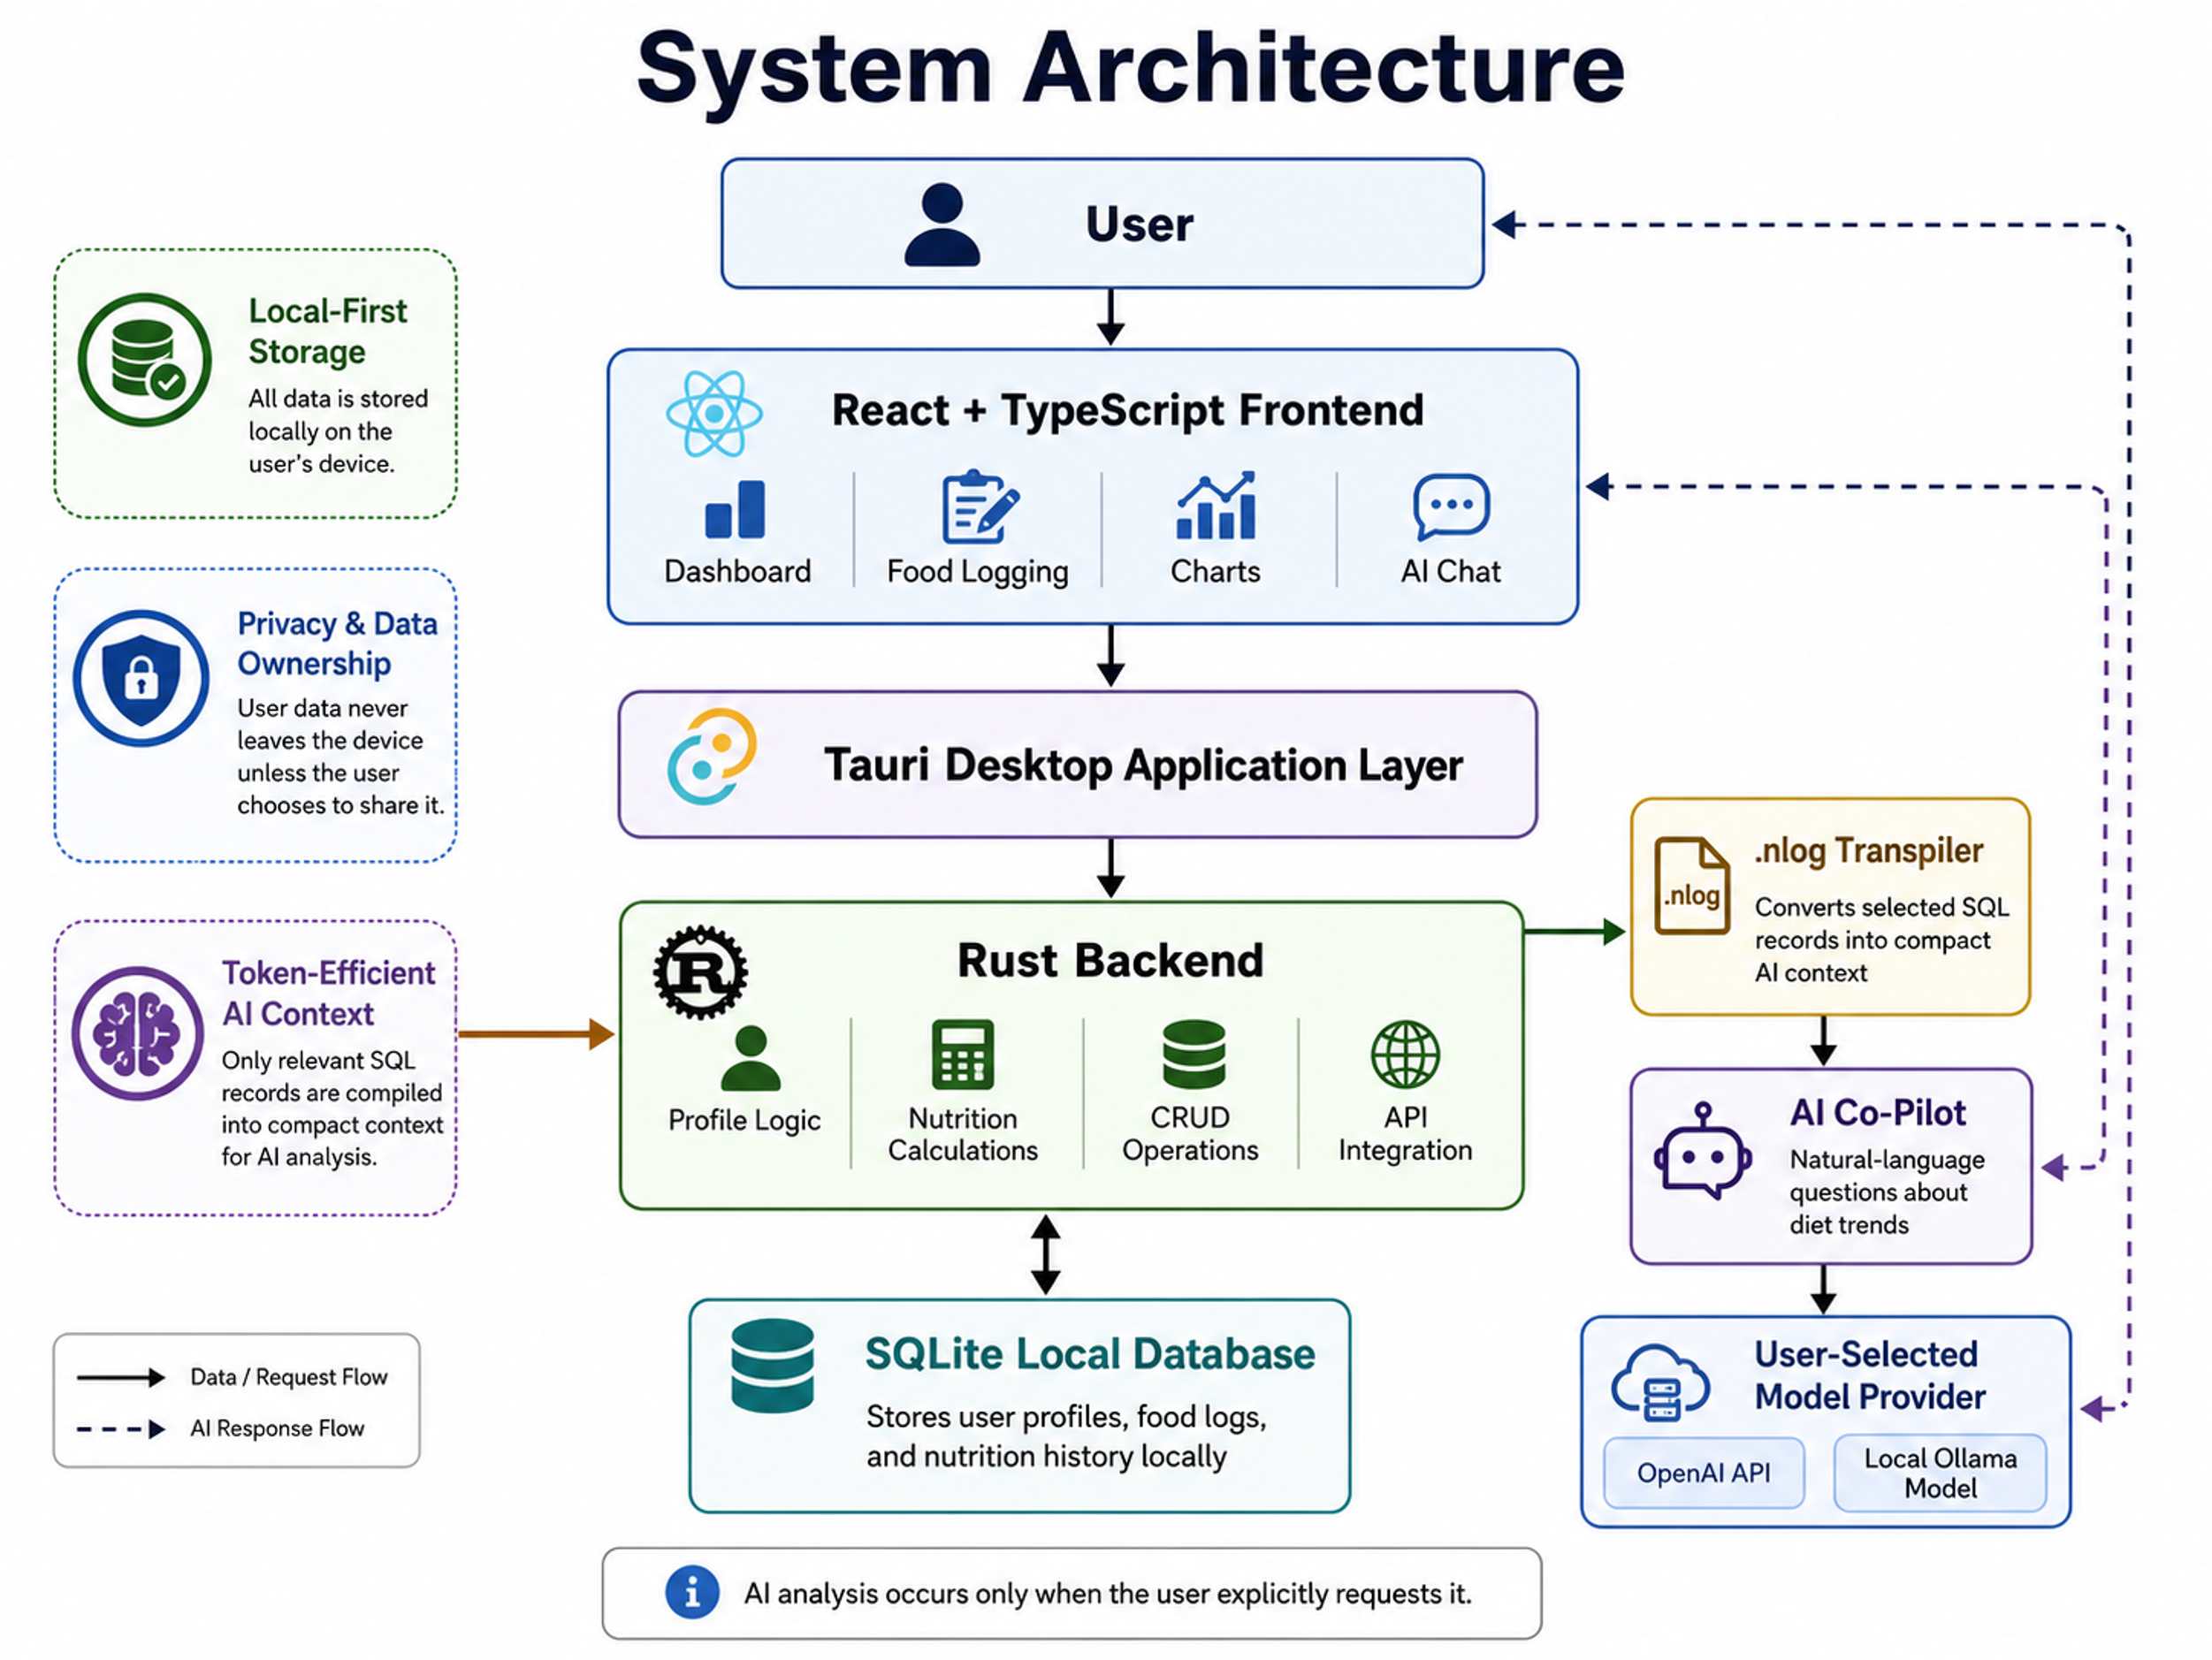
\includegraphics[width=0.95\linewidth]{images/system-design.png}
      \caption{System design for the local-first nutrition tracker.}
    \end{figure}

    \textbf{Core Design Choices:}

    \begin{itemize}
      \item \textbf{Local-first storage:} Nutrition logs and profiles stay in SQLite on the user’s device.
      \item \textbf{Bring Your Own Model:} Users can connect OpenAI or local Ollama instead of being locked into one vendor.
      \item \textbf{AI advisor pipeline:} Chat sessions, profile context, and saved history power the advisor without cloud lock-in.
      \item \textbf{\texttt{.nlog} transpiler:} Converts SQL nutrition records into compact AI-ready context.
      \item \textbf{Tauri + Rust backend:} Lightweight desktop app with fast local processing.
      \item \textbf{React + TypeScript frontend:} Clean dashboard for logging, charts, and AI interaction.
    \end{itemize}

  \end{block}

\end{column}

\separatorcolumn

\begin{column}{0.3\paperwidth}

  \begin{block}{Results}

    The insights dashboard surfaces anomalies (high sodium, low fiber) detected by threshold alerts. The local-first architecture keeps all nutrition data on-device; only user-selected context windows are sent to the AI advisor. This design preserves privacy while still enabling intelligent nutrition guidance.

    \begin{figure}
      \centering
      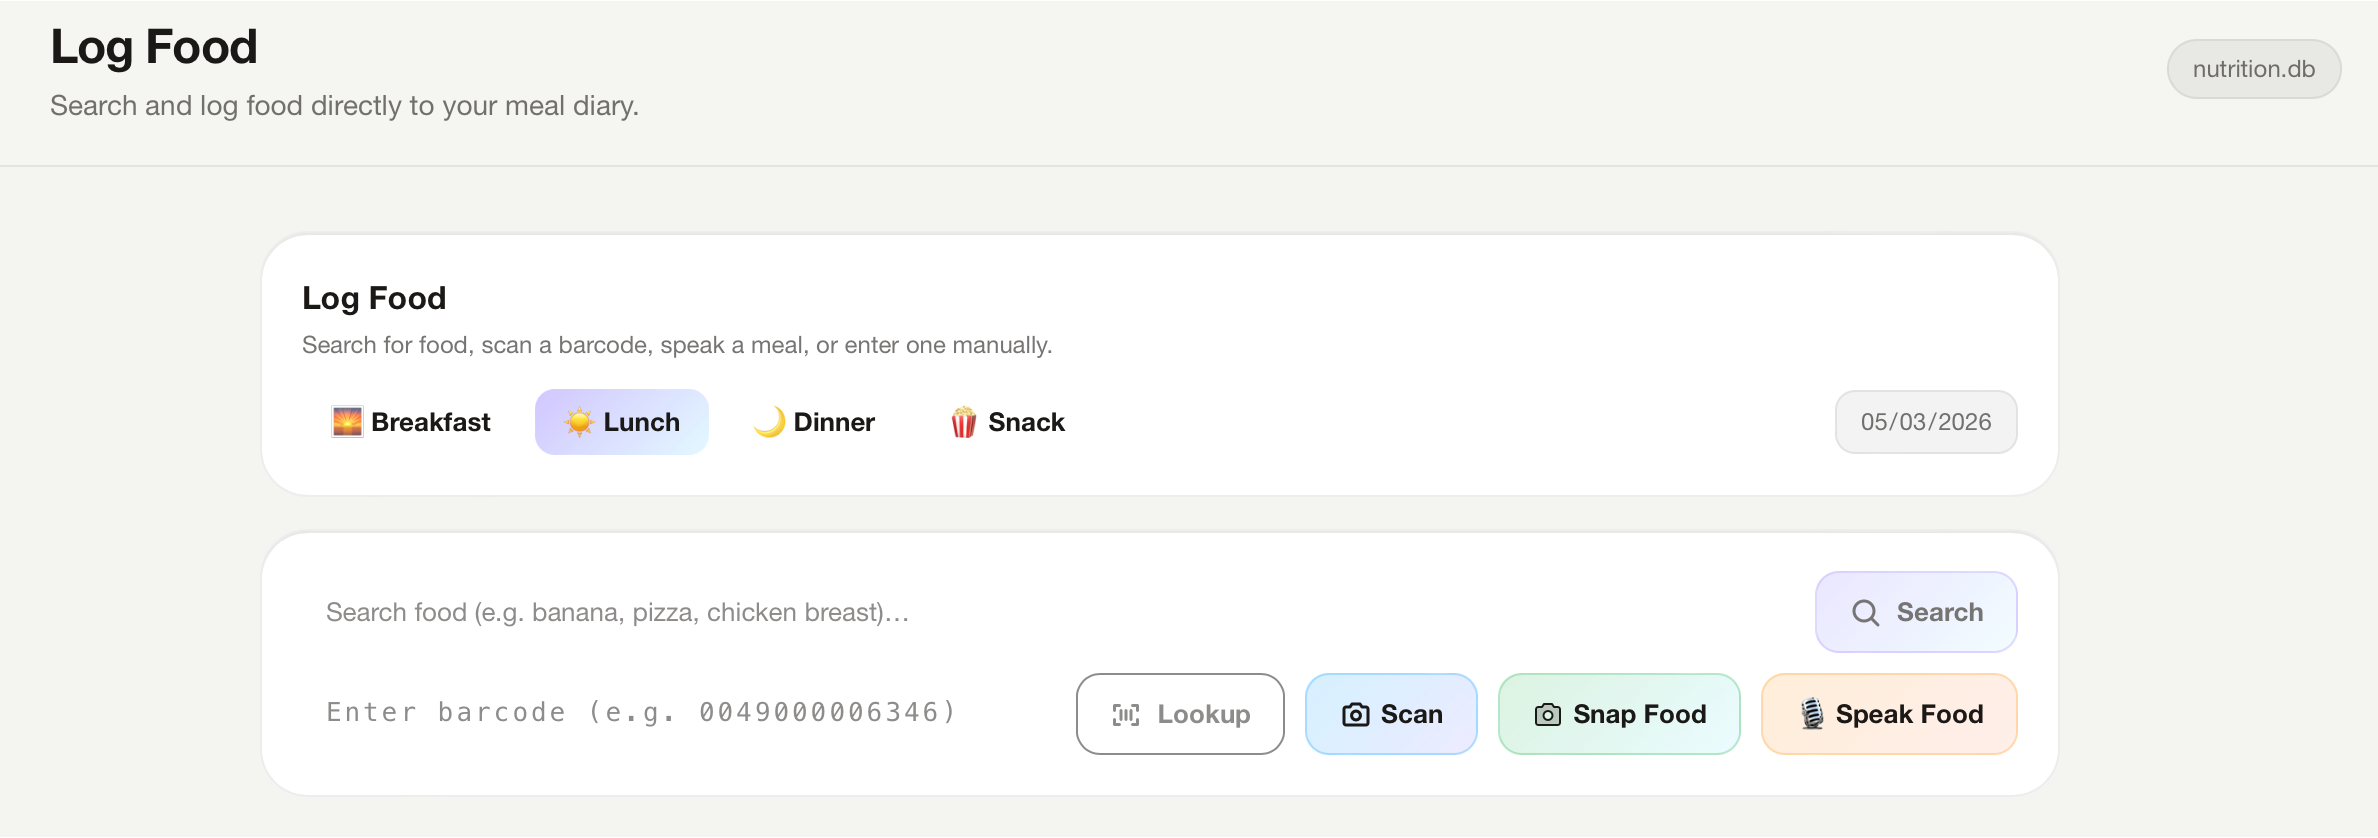
\includegraphics[width=0.9\linewidth]{images/log-food.png}
      \caption{Different ways to log food.}
      \label{fig:log-food}
    \end{figure}

    \begin{figure}
      \centering
      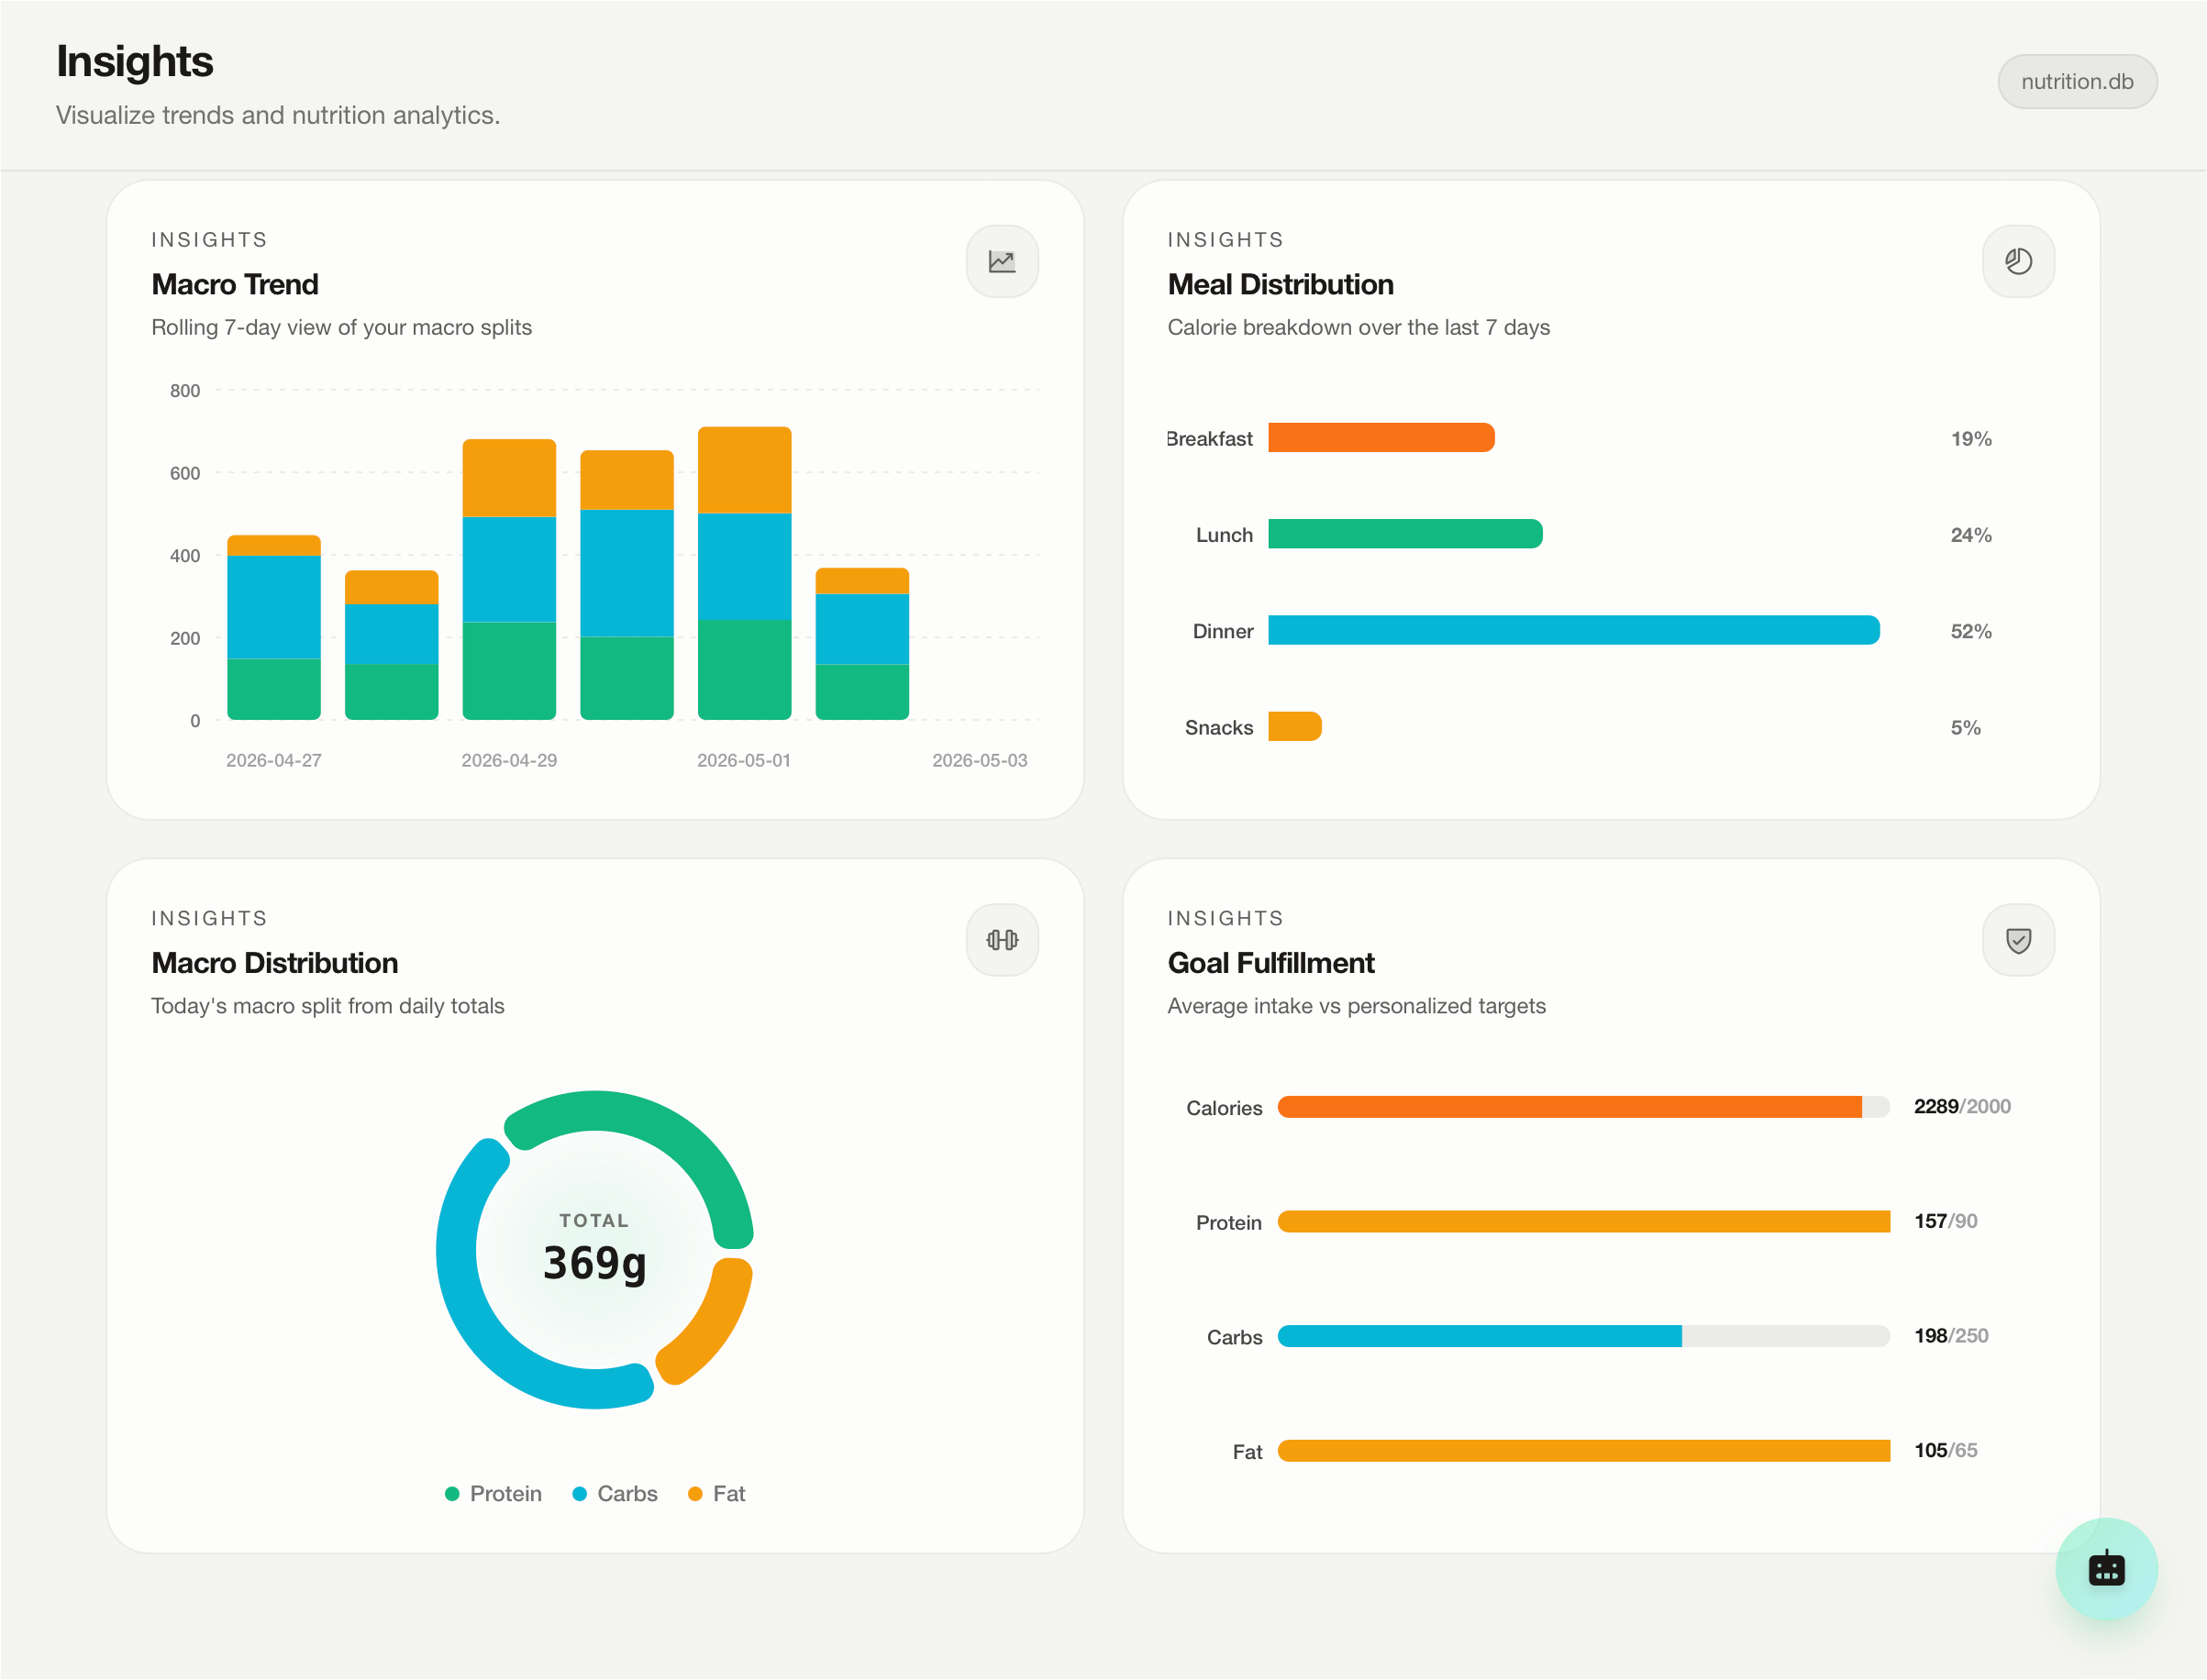
\includegraphics[width=0.9\linewidth]{images/insights.png}
      \caption{Insights dashboard with daily totals, threshold alerts, and 7-day nutrition trends.}
      \label{fig:insights}
    \end{figure}

    \begin{figure}
      \centering
      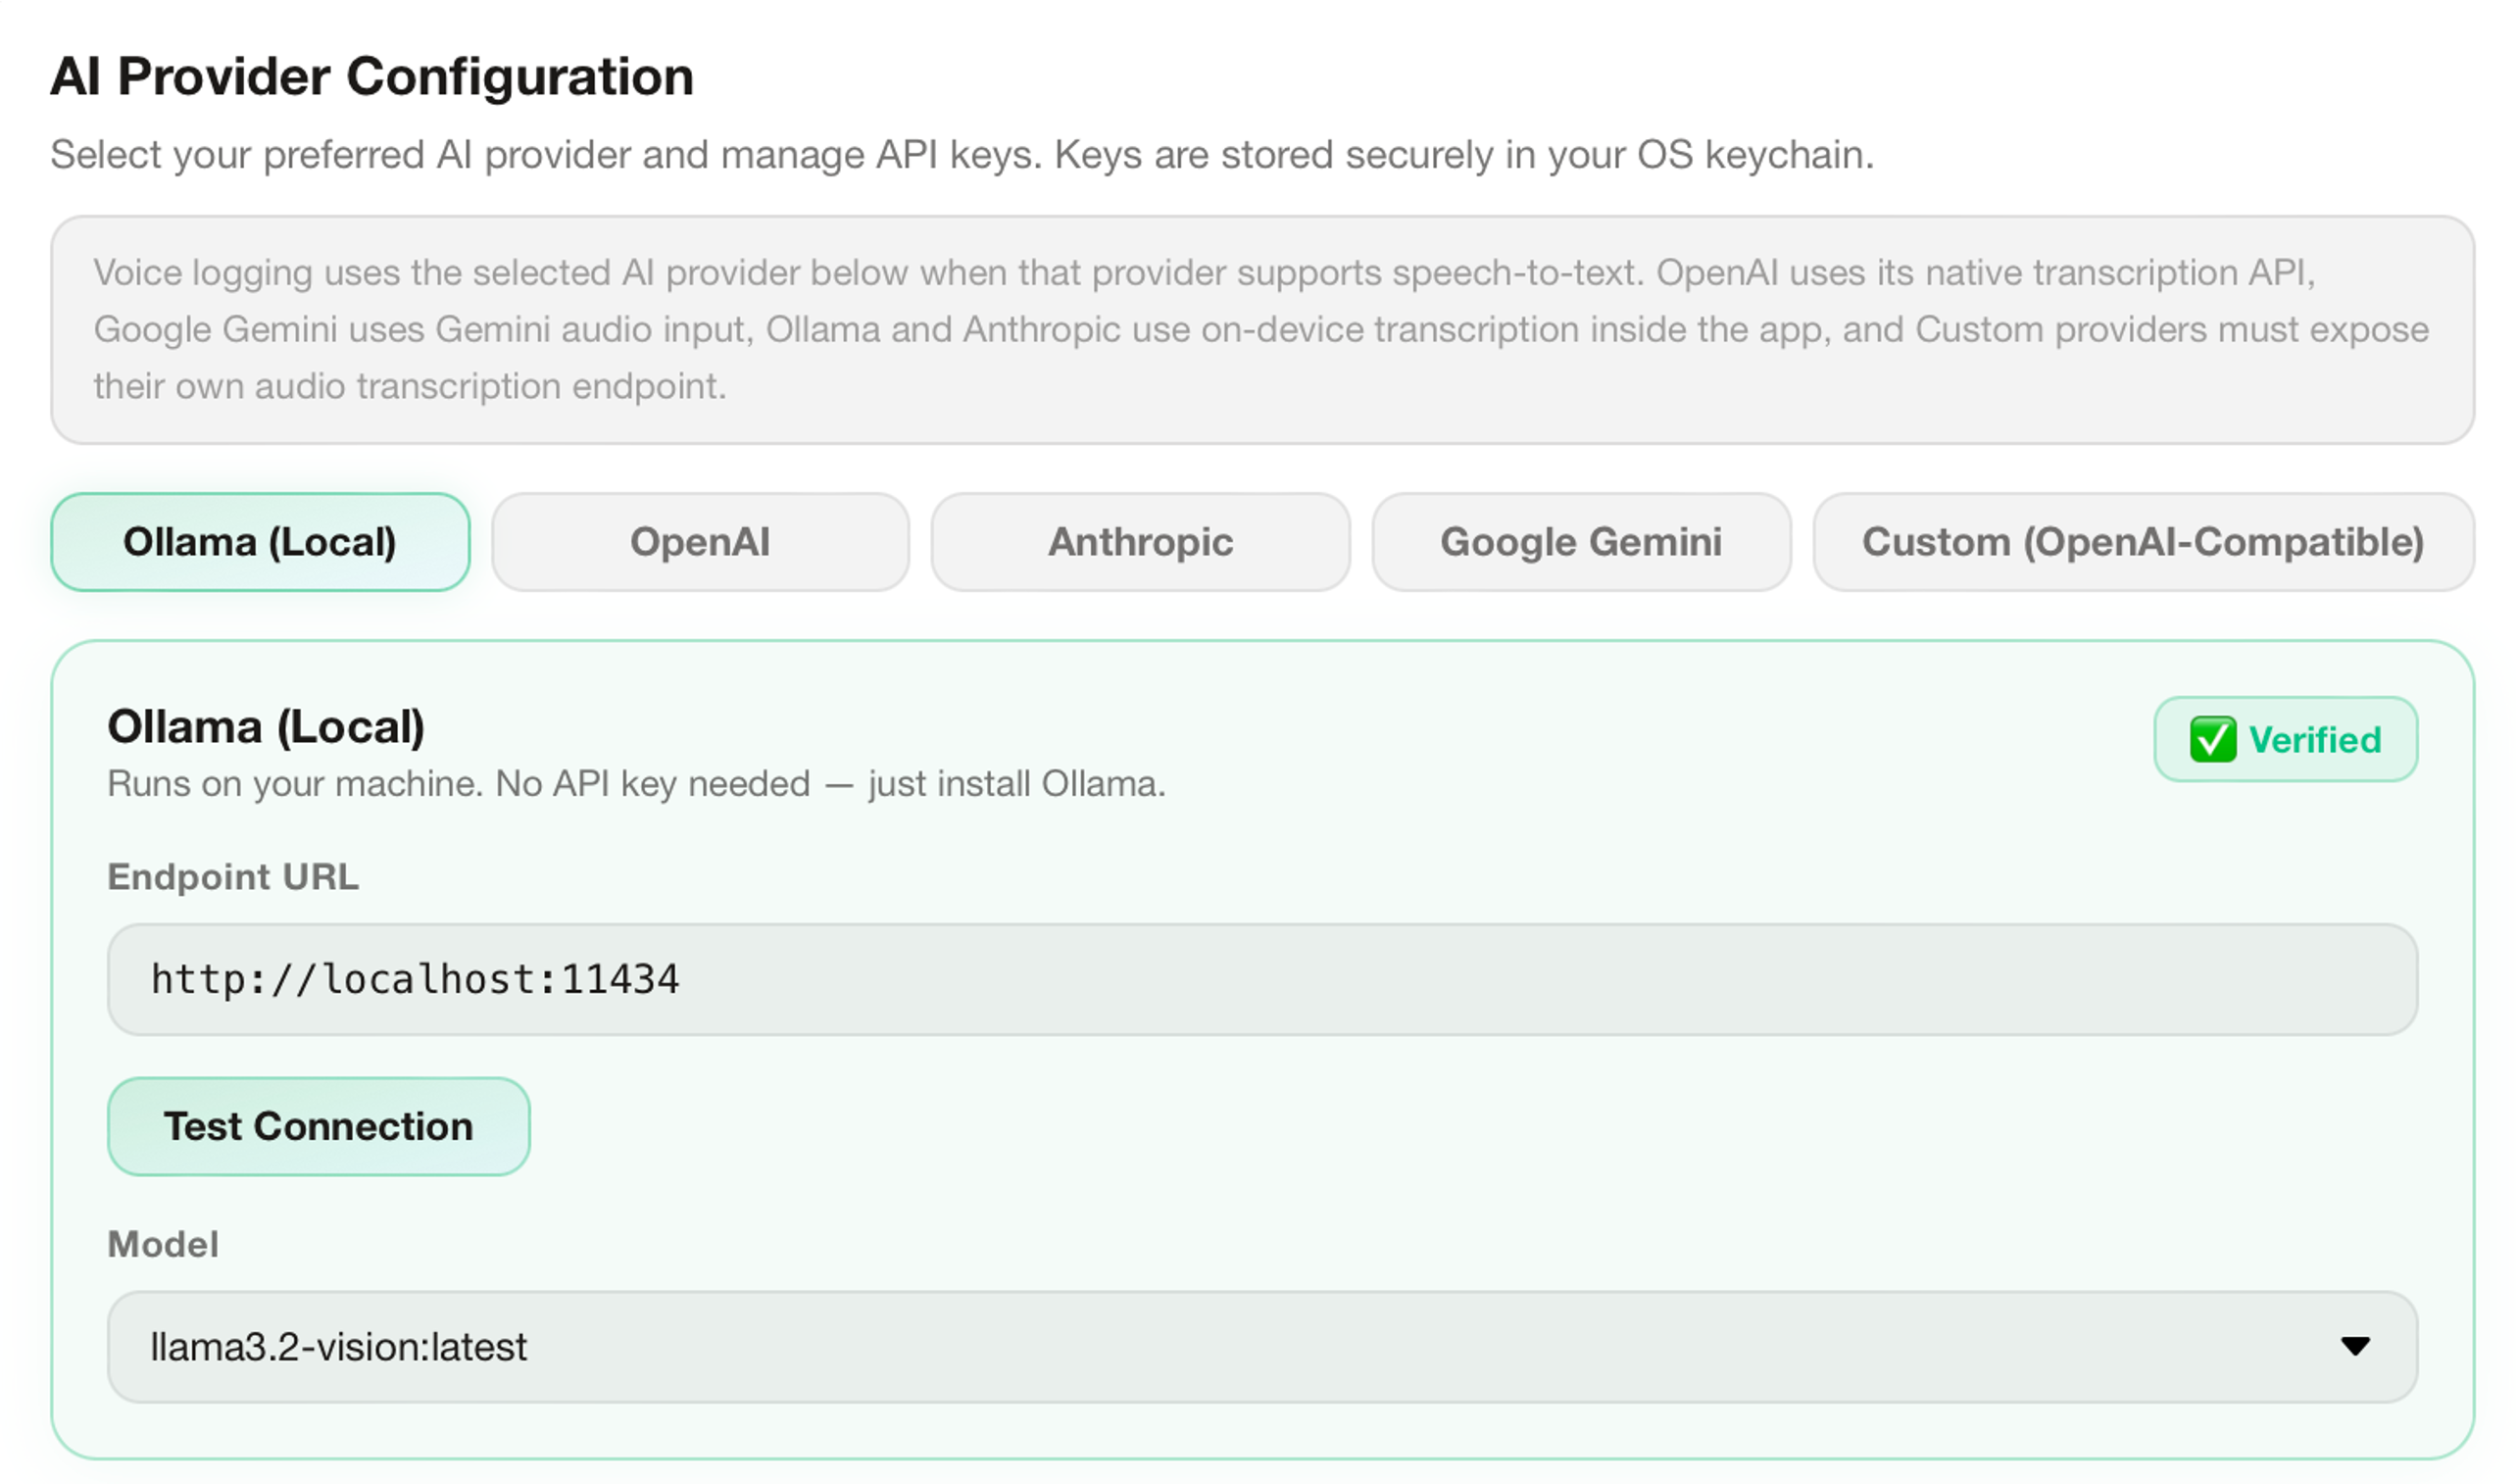
\includegraphics[width=0.9\linewidth]{images/local-first.png}
      \caption{Local-first stack: SQLite stores meals on-device; AI calls made only for specific context.}
      \label{fig:local-first}
    \end{figure}

  \end{block}

\end{column}

\separatorcolumn

\begin{column}{0.3\paperwidth}

  \begin{block}{Results (cont.)}
    
    \begin{figure}
      \centering
      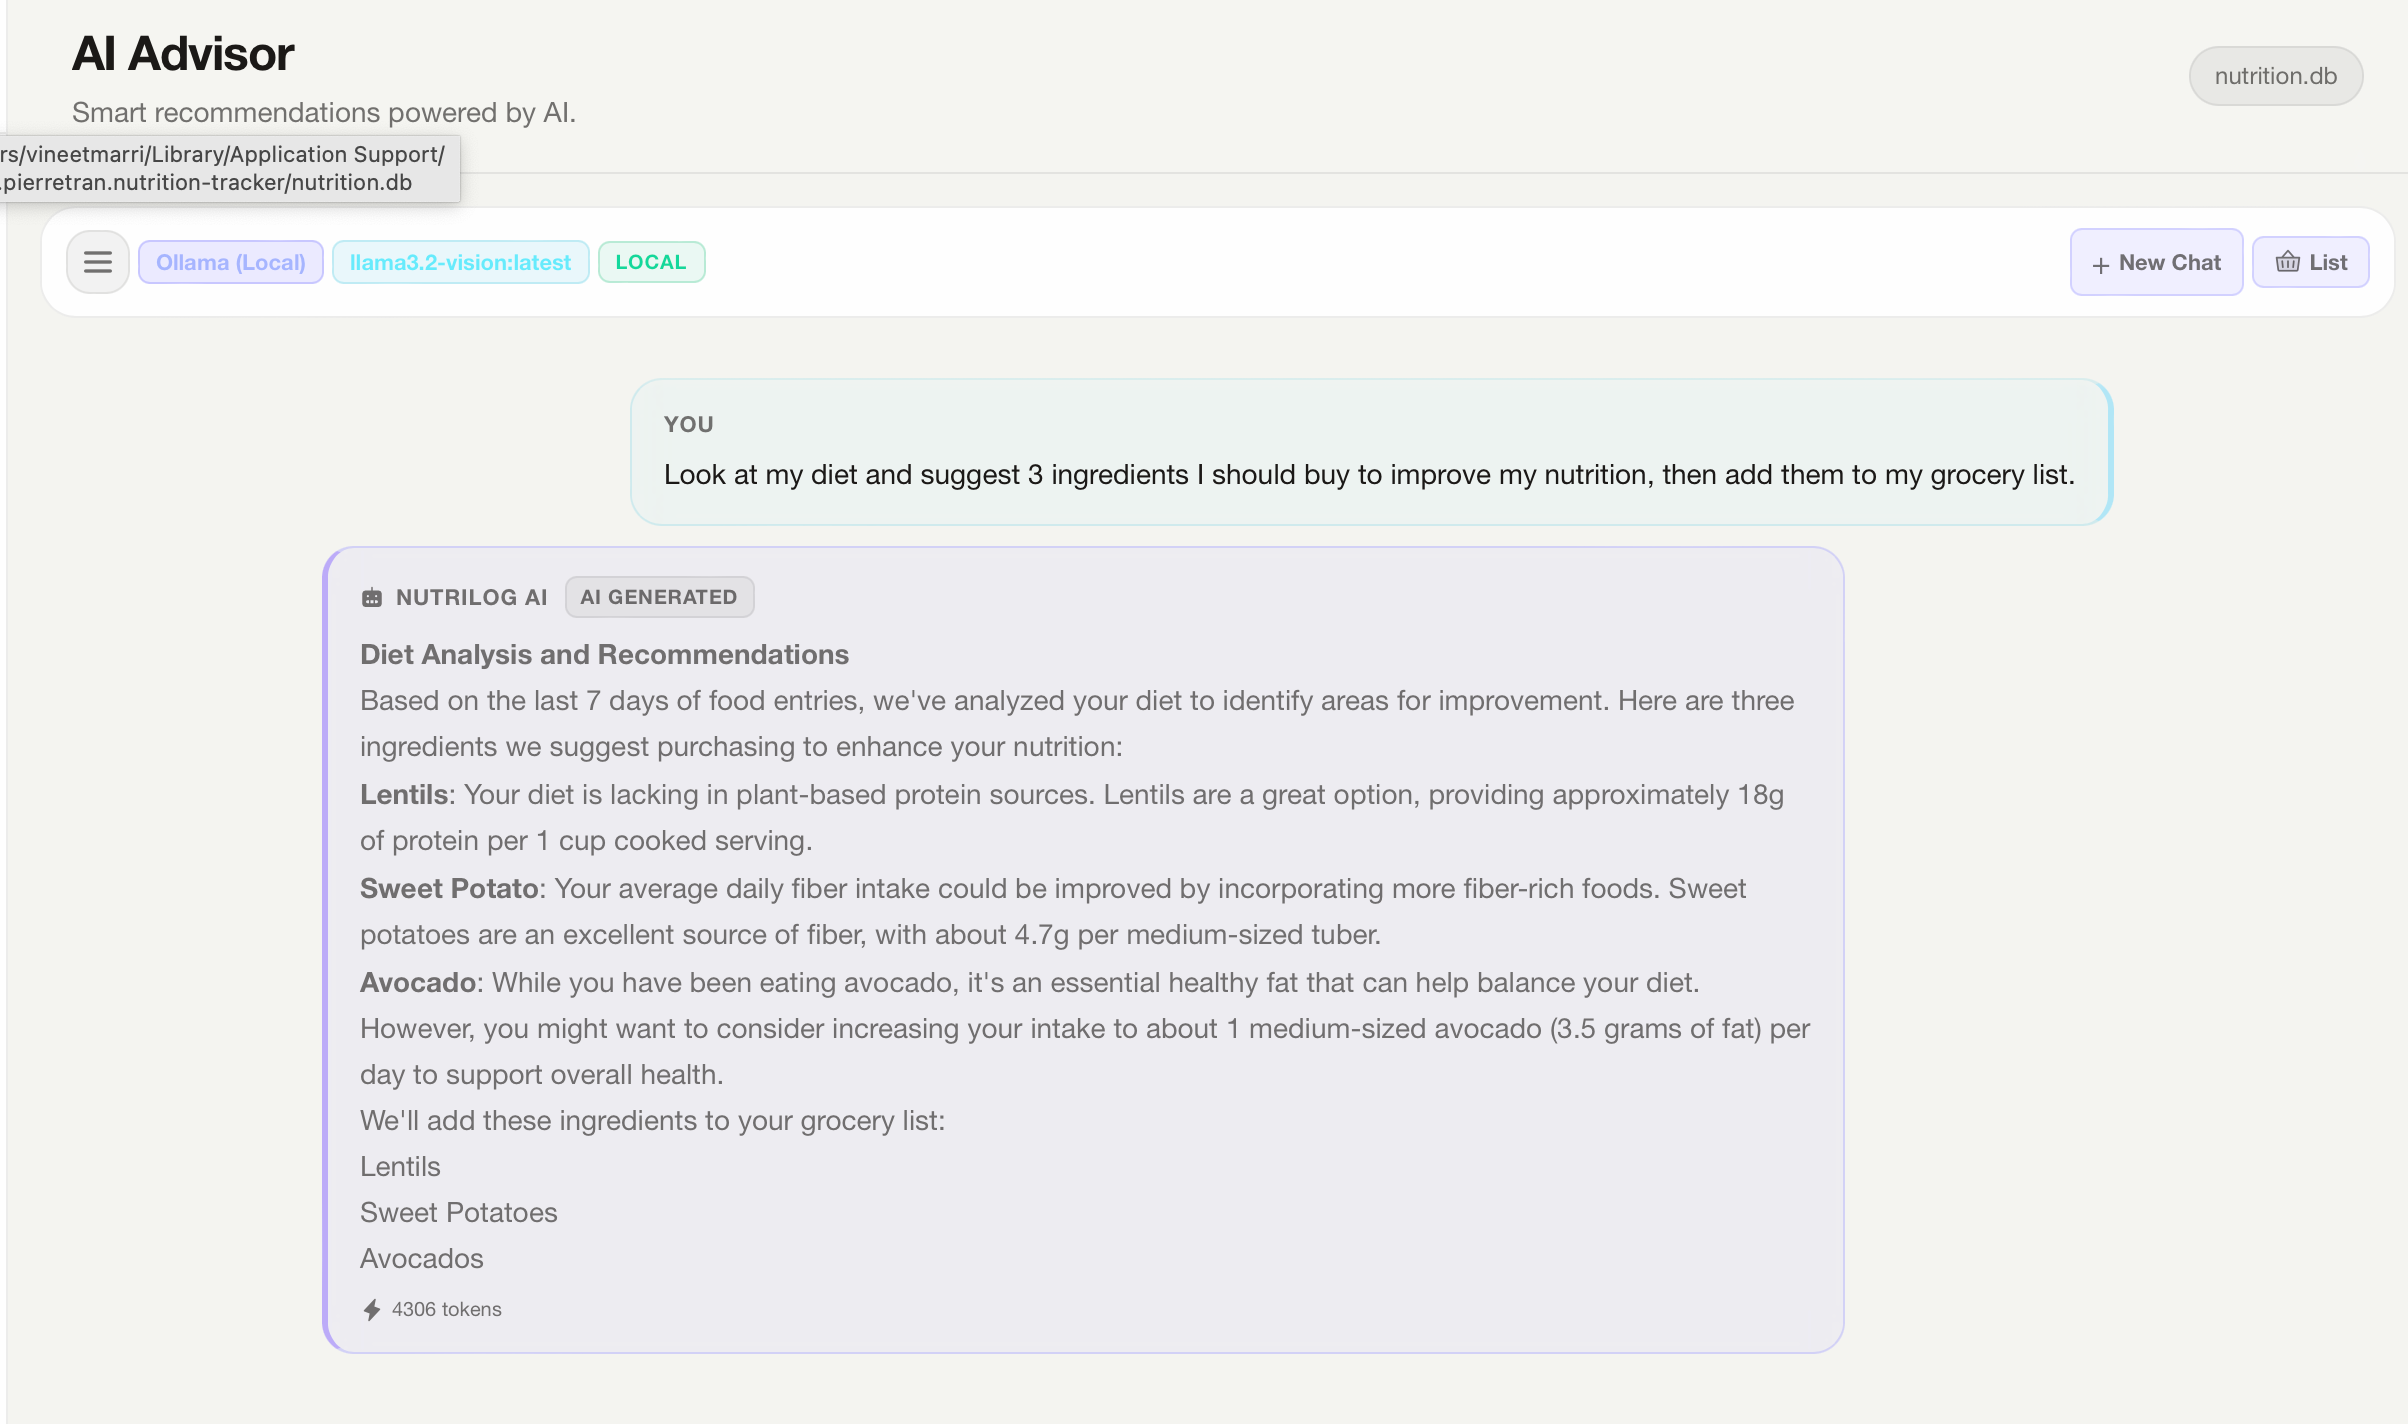
\includegraphics[width=0.8\linewidth]{images/ai-advisor.png}
      \caption{AI advisor capabilities.}
      \label{fig:ai-advisor}
    \end{figure}

    \textbf{Key Learnings \& Challenges Resolved}

    \begin{itemize}
      \item \textbf{Mobile interaction friction:} iOS keyboard focus and safe-area navigation required hardened event handling; iteratively tested on device.
      \item \textbf{Hardware resource management:} Proper camera cleanup crucial for releasing OS resources; solved through React cleanup hooks and native stubs.
      \item \textbf{AI context efficiency:} Long-term history overwhelms LLM windows; fixed by restricting to user-selected date ranges and compact serialization.
      \item \textbf{Technical debt reduction:} Migrated from inline CSS to Tailwind v4 utilities, reducing bundle size while improving maintainability across 50+ components.
    \end{itemize}

  \end{block}

  \begin{block}{Conclusion}

    \begin{itemize}
      \item Local-first nutrition tracking can protect sensitive health data while still supporting useful AI features.
      \item Compact serialization through \texttt{.nlog} makes long-term nutrition analysis more practical for LLMs.
      \item User-controlled AI improves transparency and trust compared with fully cloud-based nutrition platforms.
      \item The project shows that privacy, usability, and AI assistance can coexist in one nutrition management system.
    \end{itemize}

  \end{block}

  \begin{block}{Future Work}

    \begin{itemize}
      \item Add clinician-friendly export reports.
      \item Add confidence labels for AI-generated nutrition insights.
      \item Conduct user testing and release on app-store.
    \end{itemize}

  \end{block}

  \begin{block}{Acknowledgments}

    We would like to give special thanks to Dr. Mengistu  and Dr. Cameron for their feedback throughout the semester to help us build a better project.

    % \vspace{0.5em}

    % \nocite{*}
    % \footnotesize{\bibliographystyle{plain}\bibliography{poster}}

  \end{block}

\end{column}

\separatorcolumn
\end{columns}
\end{frame}

\end{document}
